\section{Discrete Fourier Transform}

\begin{frame}{Complex Numbers Review}
  \begin{columns}
    \begin{column}{0.65\textwidth}
      \begin{itemize}
        \item The \emph{complex numbers} are pairs of real numbers
        \item with \emph{Real} and {Complex Parts}
        \item Visualize on the \emph{Complex Plane}
        \item and analogize to a 2-d vector with the L-2 norm
        \item Write in two forms:
        \begin{itemize}
          \item $a + bj$ (Cartesian)
          \item $\alpha \exp(j \phi)$ (polar)
        \end{itemize}
        and relate using Euler's formula
        \begin{equation}
          \alpha \exp(j \phi) = \alpha \cos(\phi) + j \alpha \sin(\phi)
        \end{equation}
      \end{itemize}
    \end{column}
    \begin{column}{0.35\textwidth}
      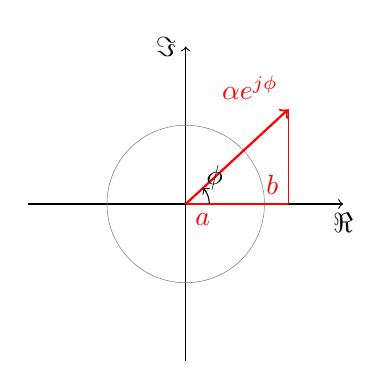
\begin{tikzpicture}
        \draw[->] (-2,0) -- (2,0) node[below] {$\Re$};
        \draw[->] (0,-2) -- (0,2) node[left] {$\Im$};
        \draw[help lines] (0,0) circle (1);

        \draw [->,red,thick] (0,0) -- (1.3,1.2) node [above left] {$\alpha e^{j \phi} $};
        \draw [red] (1.3,1.2) -- (1.3,0) node [above left] {$b$};
        \draw [red] (1.3,0) -- (0,0) node [below right] {$a$};

        \draw[->] (0:.3) arc (0:42.71:.3);
        \node at (42.71:.5) {$\phi$};
      \end{tikzpicture}
    \end{column}
  \end{columns}
\end{frame}

\begin{frame}{More Useful Formulae}
  \begin{itemize}
    \item Sinusoids to complex exponentials:
    \begin{equation}
      \cos(x) = \frac{e^{jx}+e^{-jx}}{2}
    \end{equation}
    \begin{equation}
      \sin(x) = \frac{e^{jx}-e^{-jx}}{2j}
    \end{equation}
  \item Complex Inner Product:
    \begin{equation*}
      \innerproduct{x}{y} = y^* x
    \end{equation*}
    \begin{equation*}
      \norm{x}_2^2 = \innerproduct{x}{x} 
    \end{equation*}
  \end{itemize}
\end{frame}

\begin{frame}{Roots of Unity}
  \def\n{5}
  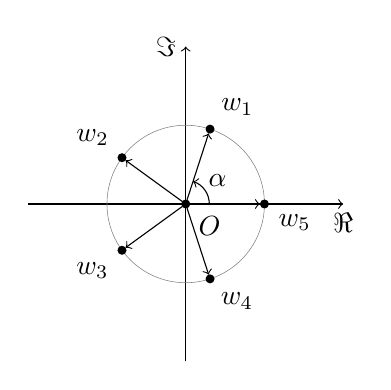
\begin{tikzpicture}[
  dot/.style={draw,fill,circle,inner sep=1pt}
  ]
  \draw[->] (-2,0) -- (2,0) node[below] {$\Re$};
  \draw[->] (0,-2) -- (0,2) node[left] {$\Im$};
  \draw[help lines] (0,0) circle (1);

  \node[dot,label={below right:$O$}] (O) at (0,0) {};
  \foreach \i in {1,...,\n} {
    \node[dot,label={\i*360/\n-(\i==\n)*45:$w_{\i}$}] (w\i) at (\i*360/\n:1) {};
    \draw[->] (O) -- (w\i);
  }
  \draw[->] (0:.3) arc (0:360/\n:.3);
  \node at (360/\n/2:.5) {$\alpha$};
\end{tikzpicture}
\end{frame}

\begin{frame}{Roots of Unity}
  \begin{itemize}
    \item \vocab{N\textsuperscript{th} root of unity} $\omega_N$ is defined to satisfy
      \begin{equation*}
        (\omega_N)^N = 1
      \end{equation*}
    \item $N$ numbers sweeping around the complex unit circle satisfy this:
      \begin{equation*}
        \omega_{k,N} = e^{j \frac{2 \pi k}{N}}
      \end{equation*}
    \item Noting that the $k$ can be pulled out of the exponent, this can also be written
      \begin{equation*}
        \omega_N^k
      \end{equation*}
  \end{itemize}
\end{frame}

\begin{frame}{DFT (Discrete Fourier Transform) Basics}
  \begin{itemize}
    \item Transforms between time- and frequency-domains
    \item N-dimensional space to N-dimensional space
    \item Orthonormal basis: $U^*U = UU^* = I$
    \item DFT is a basis of \vocab{harmonics}: $u_n[k] = \frac{1}{\sqrt{N}} \omega_N^{nk} $ which oscillate around the complex circle
  \end{itemize}
  \begin{equation*}
    U = \frac{1}{\sqrt{N}}
    \begin{pmatrix}
      1 & 1 & 1 & \ldots & 1 \\
      1 & \omega & \omega^2 & \ldots & \omega^{n-1} \\
      1 & \omega^2 & \omega^4 & \ldots  & \omega^{2(n-1)} \\
      \vdots & \vdots & \vdots & & \vdots \\
      1 & \omega^{n-1} & \omega^{2(n-1)} & \ldots & \omega^{(n-1)(n-1)} \\
    \end{pmatrix}
  \end{equation*}
\end{frame}

\begin{frame}{DFT (Discrete Fourier Transform) Basics}
  Use $U$ to transform from the frequency domain to the time domain, and use
  $F_N = U^{-1} = U^*$ to transform from the time domain to frequency.

  \begin{equation*}
    F_N = \frac{1}{\sqrt{N}}
    \begin{pmatrix}
      1 & 1 & 1 & \ldots & 1 \\
      1 & \omega^{-1} & \omega^{-2} & \ldots & \omega^{-(n-1)} \\
      1 & \omega^{-2} & \omega^{-4} & \ldots  & \omega^{-2(n-1)} \\
      \vdots & \vdots & \vdots & & \vdots \\
      1 & \omega^{-(n-1)} & \omega^{2(n-1)} & \ldots & \omega^{-(n-1)(n-1)} \\
    \end{pmatrix}
  \end{equation*}
\end{frame}

\begin{frame}{Using the DFT (Discrete Fourier Transform)}
  \begin{tikzpicture}
    \tikzstyle{block} = [rectangle, draw, fill=blue!20, 
    text width=8em, text centered, rounded corners, minimum height=4em,
    node distance=10em]
    \tikzstyle{line} = [draw, -latex']
    \node at (0,2) [block] (time-domain) {$\vec{x}$ (Time Domain)};
    \node at (0,-2)[block] (freq-domain) {$\vec{X}$ (Frequency Domain)};

    \path [line] (time-domain) -| node [left]{$F_N = U^*$} (-2,0) |- (freq-domain);
    \path [line] (freq-domain) -| node [right]{$F_N^{-1} = U$} (2,0) |- (time-domain);
  \end{tikzpicture}
\end{frame}

%%%TODO: adapt GSlide 118 is applicible

\begin{frame}{Systems in the (Discrete) Time Domain}
  \begin{itemize}
    \item Reminder: a \vocab{system} connects inputs and outputs by solving a non-homogenous differential (difference in discrete time) equation
    \item Equivalent to \vocab{convolving} an \vocab{impulse response} over the input
  \end{itemize}

  \begin{center}
  \begin{tikzpicture}
    \node at (0,0) [left] (x) {$\vec{x}[t]$};
    \node at (2,0) [draw, rectangle] (H) {$H$};
    \node at (4,0) [right] (y) {$\vec{y}[t]$};

    \draw [-latex'] (x) -- (H);
    \draw [-latex'] (H) -- (y);
  \end{tikzpicture}
  \end{center}

  \begin{equation*}
    C_{\vec{h}} \vec{x} = \vec{y}
  \end{equation*}
  where the \vocab{Circulant Matrix} for the convolution with $\vec{h}$ is written
  \begin{equation*}
    C_{\vec{h}}
    =
    \begin{pmatrix}
      h[0] & h[n-1] & \ldots & h[1] \\
      h[1] & h[0]   & \ldots & h[2] \\
      \vdots    & \vdots      & \vdots & \vdots    \\
      h[n-1] & h[n-2] & \ldots h[0] \\
    \end{pmatrix}
  \end{equation*}
\end{frame}

\begin{frame}{Systems in the (Discrete) Time Domain}
  \begin{itemize}
    \item Solve systems by \vocab{convolving} an \vocab{impulse response} over the input
    \begin{equation*}
      C_{\vec{h}} \vec{x} = \vec{y}
    \end{equation*}
  \item This is a matrix-vector multiply, $O(N^2)$.
  \item Is there a better way?
  \end{itemize}
\end{frame}

\begin{frame}{Systems in the Frequency Domain}
  \begin{itemize}
    \item If it's hard it time domain, do it in frequency!
  \end{itemize}

  \begin{center}
  \begin{tikzpicture}
    \node at (0,0) [left] (x) {$\vec{x}[t]$};
    \node at (2,0) [draw, rectangle] (H) {$H$};
    \node at (4,0) [right] (y) {$\vec{y}[t]$};

    \draw [-latex'] (x) -- (H);
    \draw [-latex'] (H) -- (y);
  \end{tikzpicture}
  \end{center}

  \begin{align*}
    U^*\vec{x} = \vec{X} && C_{\vec{h}} = U \Lambda U^* \\
  \end{align*}
  \begin{equation*}
    Y = \Lambda X
  \end{equation*}
  \begin{itemize}
    \item Matrix is diagonal in the DFT basis, find $Y$ by simple scalar multiplication, $O(n)$.
    \item Still need to move data to/from frequency domain, but the FFT (see EE123) does this in $O(n \log n)$.
  \end{itemize}
\end{frame}

\begin{frame}{Amplitude and Phase Response}
  \begin{itemize}
    \item How to systems respond to real signals?
    \item Complex exponentials are \vocab{eigenfunctions} of a system.
  \end{itemize}
  \begin{tikzpicture}
    \node at (0,0) [left] (inexp) {$\exp(j k \frac{2 \pi }{N}t)$};
    \node at (1.5,0) [draw, rectangle] (Hexp) {$H$};
    \node at (3,0) [right] (outexp) {$\lambda_k \exp(j k \frac{2 \pi}{N}t)$};

    \node at (0,-1) [left] (incos) {$\cos(k \frac{2 \pi }{N}t)$};
    \node at (1.5,-1) [draw, rectangle] (Hcos) {$H$};
    \node at (3,-1) [right] (outcos) {$\lambda_k \cos(k \frac{2 \pi}{N}t) = \abs{\lambda_k}\cos(k \frac{2\pi}{N}t + \angle \lambda_k)$};

    \draw [-latex'] (inexp) -- (Hexp);
    \draw [-latex'] (Hexp) -- (outexp);

    \draw [-latex'] (incos) -- (Hcos);
    \draw [-latex'] (Hcos) -- (outcos);
  \end{tikzpicture}

  where $\lambda_k$ is the $k$-th eigenvalue of $C_{\vec{h}}$.

  $\abs{\lambda_k}$: \vocab{magnitude response}, $\angle \lambda_k$: \vocab{phase response}
\end{frame}

\begin{frame}{Conjugate Symmetry \& Parseval's Theorem}
  \begin{itemize}
    \item The DFT basis vectors are \vocab{conjugate symmetric}:
      \begin{equation*}
        \vec{u}_k = \vec{u}_{N-k}^*
      \end{equation*}
    \item If a time-domain signal is real, is DFT-domain representation is conjugate-symmetric
      \begin{equation*}
        x[t] \in \Re \implies X[k] = \bar{X[-k]} = \var{X[N-k]}
      \end{equation*}
    \item Parseval's Theorem: Since the DFT matrix is orthonormal (and therefore unitary), ``energy'' in conserved:
      \begin{equation*}
        \norm{\vec{x}}_2 = \norm{\vec{X}}_2
      \end{equation*}
  \end{itemize}
\end{frame}

\begin{frame}{DFT True/False}
	\begin{enumerate}
	    \item<1-> The columns of the DFT matrix are orthonormal \\
	    \onslide<2->{\textbf{True}}
	    \item<1-> The DFT matrix is conjugate-symmetric \\
	    \onslide<3->{\textbf{True}}
    \item<1-> $\norm{\vec{u}_k}_2 = \sqrt{N} $\\
	    \onslide<4->{\textbf{False. That's the points of the scaling factor in our definition of the basis elements.}}
	\end{enumerate}
\end{frame}

\begin{frame}{Samling and DFT of Sinusoids}
  \begin{itemize}
    \item If we have a sinusoidal signal in the form $A \cos(\frac{2\pi}{N}(kt) + \varphi)$, we can form a time-domain vector $\vec{x}$ by sampling it
      at $N$ locations.
    \item If you take the DFT of this vector ($\vec{X} = F_N \vec{x}$), you will find only the $k$-th and $N-k$-th slots non-zero.
      Specifically, they'll take value $A \frac{\sqrt{N}}{2}\exp(j \varphi)$ (check Parseval's theorem with this!).
    \item If there is a DC offset to the signal, $\frac{X[0]}{\sqrt{N}}$ will be equal to it.
  \end{itemize}
\end{frame}

\begin{frame}{DFT Practice Problem Warmup}
  Find the DFT coefficients for the following $N=8$ signal:
  \begin{equation*}
    x[t] = e^{j\frac{\pi}{2}t} + e^{j\frac{3\pi}{2}t}
  \end{equation*}

  \pause Hint: put into form from previous slide.

\end{frame}

\begin{frame}{DFT Practice Problem Warmup Solution}
  \begin{align*}
    x[t] &=  e^{j\frac{\pi}{2}t} + e^{j\frac{3\pi}{2}t} \\
    &= e^{j\pi t} (e^{-j\frac{\pi}{2}t} + e^{j\frac{\pi}{2}t}) \\
    &= (-1)^t \cos(\frac{4\pi}{8} t) \\
  \end{align*}
\end{frame}

